\documentclass[handout]{beamer}
\usetheme{metropolis}
\beamertemplatetransparentcoveredhigh

\usepackage[portuges]{babel}
\usepackage{graphicx}
\graphicspath{{./figs/}}
\usepackage{listings}
\usepackage{color}
\usepackage{hyperref}
\usepackage{xpatch}
\usepackage{comment}
\usepackage[outputdir=build]{minted}

\makeatletter
\AtBeginEnvironment{minted}{\dontdofcolorbox}
\def\dontdofcolorbox{\renewcommand\fcolorbox[4][]{##4}}
\xpatchcmd{\inputminted}{\minted@fvset}{\minted@fvset\dontdofcolorbox}{}{}
\xpatchcmd{\mintinline}{\minted@fvset}{\minted@fvset\dontdofcolorbox}{}{}
\makeatother
\setminted[c]{
  linenos=true,
  breaklines=true,
  encoding=utf8,
  frame=lines,
  framerule=0.5pt,
  autogobble,
  fontsize=\small,
}
\setminted[bash]{
  linenos=true,
  encoding=utf8,
  frame=lines,
  framerule=0.5pt,
  autogobble,
  fontsize=\small
}

\newcommand{\cod}[1]{\mintinline{c}{#1}}


\definecolor{dkgreen}{rgb}{0,0.6,0}
\definecolor{gray}{rgb}{0.5,0.5,0.5}
\definecolor{mauve}{rgb}{0.58,0,0.82}


\definecolor{Purple}{HTML}{911146}
\definecolor{Orange}{HTML}{CF4A30}
\setbeamercolor{alerted text}{fg=Orange}
\setbeamercolor{frametitle}{bg=Purple}
\setbeamercolor{block body}{bg=Purple!20,fg=black}
\setbeamercolor{block title}{bg=Purple!50,fg=black}
\setbeamertemplate{blocks}[rounded][shadow=true]


\newcounter{ExercicioCounter}
\newcommand{\exercicio}{\refstepcounter{ExercicioCounter} Exercício~\theExercicioCounter}

\newcommand{\setcoverbg}{
  \setbeamertemplate{background}
  {
\includegraphics[width=\paperwidth,height=\paperheight]{backgrounds/coverbg}}
}
\newcommand{\setsectionbg}{
  \setbeamertemplate{background}
  {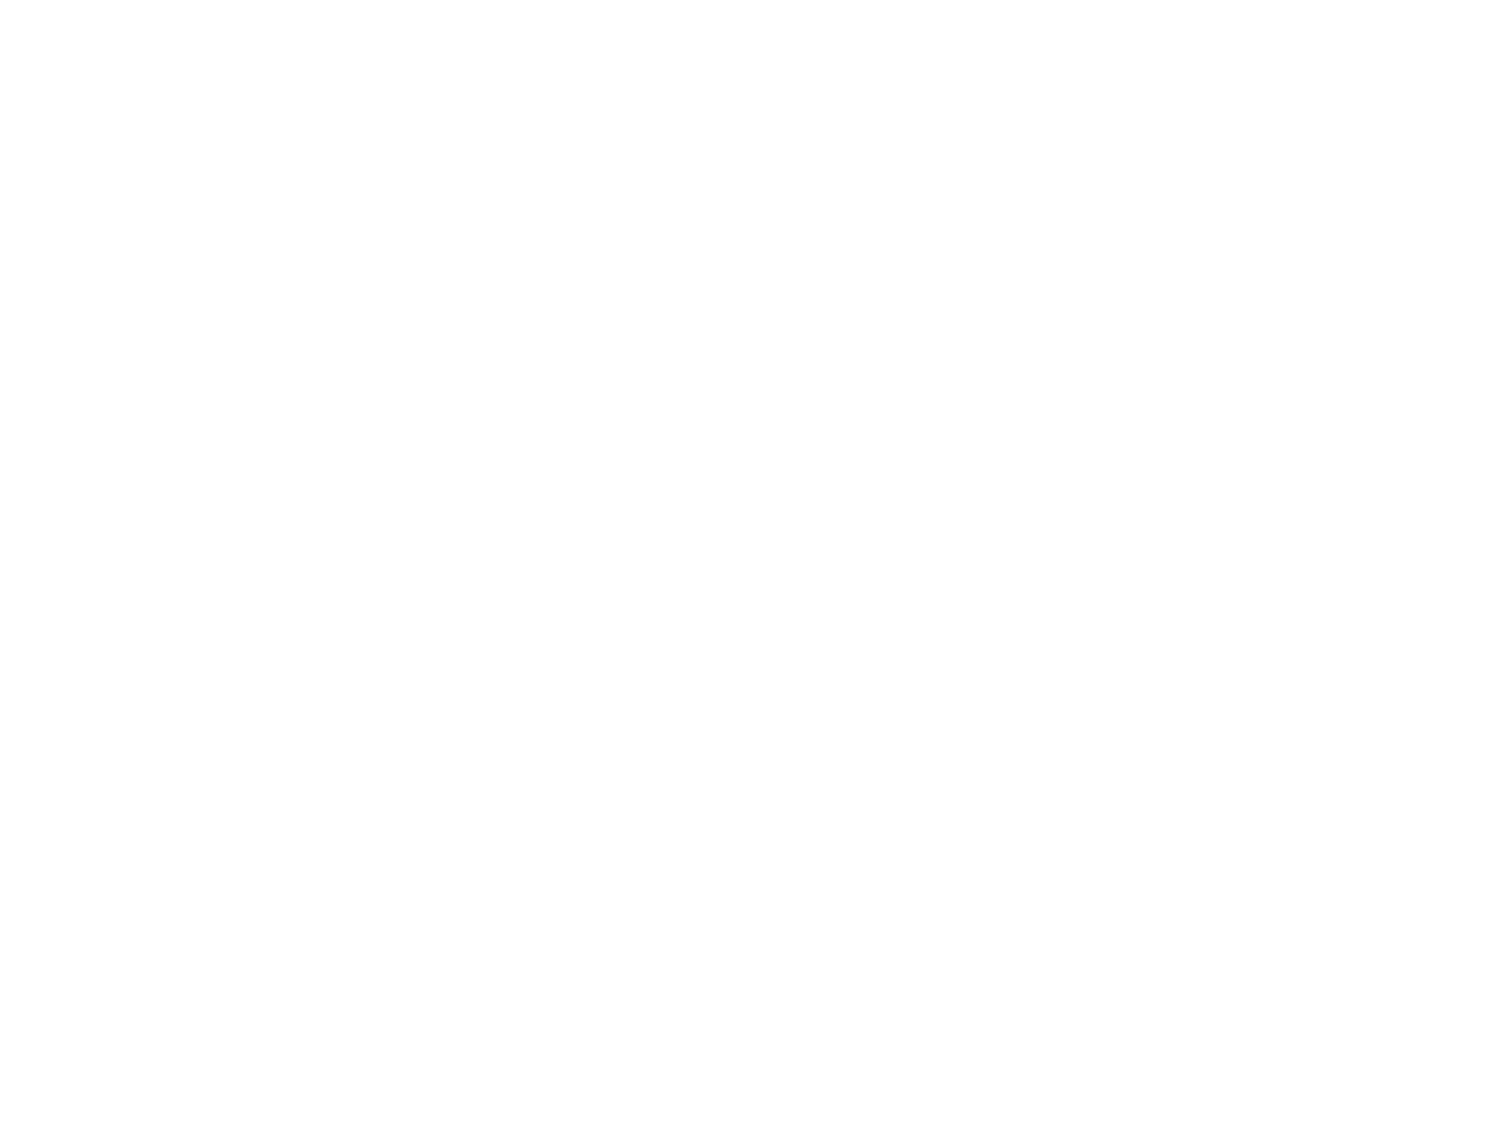
\includegraphics[width=\paperwidth,height=\paperheight]{backgrounds/blank}}
}

\title{Programação Estruturada}
\subtitle{Ordenação}

\author{Professores Emílio Francesquini e Carla Negri Lintzmayer}
\institute{Centro de Matemática, Computação e Cognição\\ Universidade Federal do ABC}
\date{2018.Q3}

\begin{document}

\setcoverbg
\maketitle
\setsectionbg


%%%%%%%%%%%%%%%%%%%%%%%%%%%%%%%%%%%%%%%%%%%%
%%%%%%%%%%%%%%%%%%%%%%%%%%%%%%%%%%%%%%%%%%%%
%%%%%%%%%%%%%%%%%%%%%%%%%%%%%%%%%%%%%%%%%%%%
%%%%%%%%%%%%%%%%%%%%%%%%%%%%%%%%%%%%%%%%%%%%
%%%%%%%%%%%%%%%%%%%%%%%%%%%%%%%%%%%%%%%%%%%%
%%%%%%%%%%%%%%%%%%%%%%%%%%%%%%%%%%%%%%%%%%%%
\section{O problema da ordenação}

%%%%%%%%%%%%%%%%%%%%%%%%%%%%%%%%%%%%
\begin{frame}[fragile]{Ordenação}

    \begin{block}{Problema}
        Dado uma coleção de elementos com uma relação de ordem entre si, devemos gerar uma saída com os elementos ordenados.
    \end{block}

    Nos nossos exemplos usaremos um vetor de inteiros para representar tal coleção.

    \begin{itemize}
        \item É claro que quaisquer inteiros possuem uma relação de ordem entre si.
    \end{itemize}

    Apesar de usarmos inteiros, os algoritmos servem para ordenar qualquer coleção de elementos que possam ser comparados.

\end{frame}

%%%%%%%%%%%%%%%%%%%%%%%%%%%%%%%%%%%%
\begin{frame}[fragile]{Ordenação}

    \begin{itemize}
        \item O problema de ordenação é um dos mais básicos em computação. 
        \begin{itemize}
            \item Mas muito provavelmente é um dos problemas com o maior número de aplicações diretas ou indiretas (como parte da solução para um problema maior).
        \end{itemize}

        \item Criar {\it rankings}
        \item Definir preferências em atendimentos por prioridade
        \item Criar listas
        \item Otimizar sistemas de busca
        \item Manter estruturas de bancos de dados
        \item Etc.
    \end{itemize}
 
\end{frame}

%%%%%%%%%%%%%%%%%%%%%%%%%%%%%%%%%%%%
\begin{frame}[fragile]{Ordenação}

    Existem \textbf{muitos} algoritmos de ordenação:
    \begin{itemize}
        \item Selection Sort
        \item Merge Sort
        \item Insertion Sort
        \item Quicksort
        \item Heapsort
        \item Bubble Sort
        \item Shell Sort
        \item Bogosort
        \item \ldots
        \item \url{https://nicholasandre.com.br/sorting/}
    \end{itemize}

\end{frame}

%%%%%%%%%%%%%%%%%%%%%%%%%%%%%%%%%%%%
%%%%%%%%%%%%%%%%%%%%%%%%%%%%%%%%%%%%
%%%%%%%%%%%%%%%%%%%%%%%%%%%%%%%%%%%%
%%%%%%%%%%%%%%%%%%%%%%%%%%%%%%%%%%%%
%%%%%%%%%%%%%%%%%%%%%%%%%%%%%%%%%%%%
%%%%%%%%%%%%%%%%%%%%%%%%%%%%%%%%%%%%
\section{Selection Sort}

%%%%%%%%%%%%%%%%%%%%%%%%%%%%%%%%%%%%
\begin{frame}[fragile]{Selection Sort}

    \begin{itemize}
        \item Seja \cod{vet} um vetor contendo números inteiros.
        \item Devemos deixar \cod{vet} em ordem crescente.
        \item A ideia do algoritmo é a seguinte:
        \begin{itemize}
            \item Ache o menor elemento a partir da posição 0. Troque então este elemento com o elemento da posição 0.
            \item Ache o menor elemento a partir da posição 1. Troque então este elemento com o elemento da posição 1.
            \item Ache o menor elemento a partir da posição 2. Troque então este elemento com o elemento da posição 2.
            \item E assim sucessivamente\ldots
        \end{itemize}
     \end{itemize}

\end{frame}

%%%%%%%%%%%%%%%%%%%%%%%%%%%%%%%%%%%%
\begin{frame}[fragile]{Selection Sort}
    
    Exemplo: (5,3,2,1,90,6).

    Iteração 0.
    Acha o menor: (5,3,2,{\color{blue}\underline{1}},90,6).\\
    Faz troca: ({\color{red}\underline{1}},3,2,{\color{red}\underline{5}},90,6).\\
    \pause
    Iteração 1.
    Acha o menor: (1,3,{\color{blue}\underline{2}},5,90,6).\\
    Faz troca: (1,{\color{red}\underline{2}},{\color{red}\underline{3}},5,90,6).\\
    \pause
    Iteração 2.
    Acha o menor: (1,2,{\color{blue}\underline{3}},5,90,6).\\
    Faz troca: (1,2,{\color{red}\underline{3}},5,90,6).\\
    \pause
    Iteração 3.
    Acha o menor: (1,2,3,{\color{blue}\underline{5}},90,6).\\
    Faz troca: (1,2,3,{\color{red}\underline{5}},90,6).\\
    \pause
    Iteração 4.
    Acha o menor: (1,2,3,5,90,{\color{blue}\underline{6}}).\\
    Faz troca: (1,2,3,5,{\color{red}\underline{6}},{\color{red}\underline{90}}).
    
\end{frame}

%%%%%%%%%%%%%%%%%%%%%%%%%%%%%%%%%%%%
\begin{frame}[fragile]{Selection Sort}

    \begin{itemize}
        \item Como achar o menor elemento a partir de uma posição inicial?
        \item Vamos achar {\bf o índice} do menor elemento em um vetor, a partir de uma posição inicial {\bf ini}:
    \end{itemize}

    \begin{minted}{c}
        int min = ini, j;
        for (j = ini+1; j < tam; j++) {
            if (vet[min] > vet[j])
                min = j;
        }
    \end{minted}

\end{frame}

%%%%%%%%%%%%%%%%%%%%%%%%%%%%%%%%%%%%
\begin{frame}[fragile]{Selection Sort}

    Criamos então uma função que retorna o índice do elemento mínimo de um vetor, a partir de uma posição {\bf ini} passada por parâmetro.

    \begin{minted}{c}
        int indiceMenor(int vet[], int tam, int ini) {
            int min = ini, j;
            for (j = ini+1; j < tam; j++) {
                if (vet[min] > vet[j])
                    min = j;
            }
            return min;
        }
    \end{minted}

\end{frame}

%%%%%%%%%%%%%%%%%%%%%%%%%%%%%%%%%%%%
\begin{frame}[fragile]{Selection Sort}

    \begin{itemize}
        \item Dada a função anterior para achar o índice do menor elemento, como implementar o algoritmo de ordenação?
        \item Ache o menor elemento a partir da posição 0, e troque com o elemento da posição 0.
        \item Ache o menor elemento a partir da posição 1, e troque com o elemento da posição 1.
        \item Ache o menor elemento a partir da posição 2, e troque com o elemento da posição 2.
        \item E assim sucessivamente\ldots
    \end{itemize}

\end{frame}

%%%%%%%%%%%%%%%%%%%%%%%%%%%%%%%%%%%%
\begin{frame}[fragile]{Selection Sort}

    \begin{minted}{c}
        void selectionSort(int vet[], int tam) {
            int i, min, aux;
            
            for (i = 0; i < tam; i++) {
                /* Acha posicao do menor elemento a partir de i */
                min = indiceMenor(vet, tam, i);
                /* Troca o menor elemento com o da posição i */
                aux = vet[i];
                vet[i] = vet[min];
                vet[min] = aux;
            }
        }
    \end{minted}

\end{frame}

%%%%%%%%%%%%%%%%%%%%%%%%%%%%%%%%%%%%
\begin{frame}[fragile]{Selection Sort}

    Com as funções anteriores podemos executar o exemplo:
    \vspace{-1em}
    \begin{minted}[fontsize=\scriptsize]{c}
        int main() {
            int vetor[10] = {14,7,8,34,56,4,0,9,-8,100};
            int i;

            printf("Vetor Antes: (%d", vetor[0]);
            for (i = 1; i < 10; i++)
                printf(", %d", vetor[i]);
            printf(")\n");

            selectionSort(vetor, 10);

            printf("Vetor Depois: (%d", vetor[0]);
            for (i = 1; i < 10; i++)
                printf(", %d", vetor[i]);
            printf(")\n");

            return 0;
        }
    \end{minted}

\end{frame}

%%%%%%%%%%%%%%%%%%%%%%%%%%%%%%%%%%%%
\begin{frame}[fragile]{Selection Sort}

    \begin{itemize}
        \item A função para achar o índice do menor elemento não é estritamente necessária.
        \item Podemos refazer a função \cod{selectionSort} como segue:
    \end{itemize}
    \vspace{-1.5em}
    \begin{minted}{c}
        void selectionSort(int vet[], int tam) {
            int i, j, min, aux;
            for (i = 0; i < tam; i++) {
                min = i;
                for (j = i+1; j < tam; j++) {
                    if (vet[min] > vet[j])
                        min = j;
                } 
                aux = vet[i];
                vet[i] = vet[min];
                vet[min] = aux;
            }
        }
    \end{minted}

\end{frame}

%%%%%%%%%%%%%%%%%%%%%%%%%%%%%%%%%%%%
\begin{frame}[fragile]{Selection Sort}
    
    Mas podemos também criar uma função troca:
    \vspace{-1em}
    \begin{minted}{c}
        void troca(int *a, int *b) {
            int aux = *a;
            *a = *b;
            *b = aux;
        }
    \end{minted}
    \pause

    E assim \cod{selectionSort} pode ser reescrita:
    \vspace{-1em}
    \begin{minted}{c}
        void selectionSort(int vet[], int tam) {
            int i, min;
            for (i = 0; i < tam; i++) {
                min = indiceMenor(vet, tam, i);
                troca(&vet[i], &vet[min]);
            }
        }
    \end{minted}

\end{frame}

%%%%%%%%%%%%%%%%%%%%%%%%%%%%%%%%%%%%
%%%%%%%%%%%%%%%%%%%%%%%%%%%%%%%%%%%%
%%%%%%%%%%%%%%%%%%%%%%%%%%%%%%%%%%%%
%%%%%%%%%%%%%%%%%%%%%%%%%%%%%%%%%%%%
%%%%%%%%%%%%%%%%%%%%%%%%%%%%%%%%%%%%
%%%%%%%%%%%%%%%%%%%%%%%%%%%%%%%%%%%%
\section{Merge Sort}

%%%%%%%%%%%%%%%%%%%%%%%%%%%%%%%%%%%%
\begin{frame}[fragile]{Merge Sort}

    \begin{itemize}
        \item Seja \cod{vet} um vetor contendo \cod{tam} números inteiros.
        \item Devemos deixar \cod{vet} em ordem crescente.
        \item E se soubéssemos ordenar vetores de tamanho menor?
    \end{itemize}

\end{frame}

%%%%%%%%%%%%%%%%%%%%%%%%%%%%%%%%%%%%
\begin{frame}[fragile]{Merge Sort}

    \begin{itemize}
        \item Suponha que temos dois vetores \cod{A} e \cod{B} de tamanho \cod{tam/2} cada que já estão em ordem crescente.
        \item Como podemos colocá-los em um único vetor \cod{vet} de tamanho \cod{tam} totalmente ordenado?
    \end{itemize}

    $$(3,5,7,10,25,36) \qquad (1,2,6,13,17,28)$$

    \begin{itemize}
        \item Qual elemento vai ficar em \cod{vet[0]}?
    \end{itemize}

\end{frame}

%%%%%%%%%%%%%%%%%%%%%%%%%%%%%%%%%%%%
\begin{frame}[fragile]{Merge Sort}
    
    \begin{itemize}
        \item Em \cod{vet[0]} só podemos ter \cod{A[0]} ou \cod{B[0]}, o que for menor dentre esses dois.
        \item Se \cod{vet[0] = A[0]}, então \cod{vet[1]} só pode ter \cod{A[1]} ou \cod{B[0]}, o que for menor dentre esses dois.
        \item Mas se \cod{vet[0] = B[0]}, então \cod{vet[1]} só pode ter \cod{A[0]} ou \cod{B[1]}, o que for menor dentre esses dois.
        \item Note que uma vez que um elemento \cod{A[i]} é copiado para \cod{vet}, esse elemento não deve mais ser considerado (comparado com um elemento de \cod{B}).
        \item Da mesma forma, uma vez que um elemento \cod{B[j]} é copiado para \cod{vet}, esse elemento não deve mais ser considerado (comparado com um elemento de \cod{A}).
    \end{itemize}

\end{frame}

%%%%%%%%%%%%%%%%%%%%%%%%%%%%%%%%%%%%
\begin{frame}[fragile]{Merge Sort}

    Precisamos manter:
    \begin{itemize}
        \item Um índice \cod{i} para percorrer o vetor \cod{A}.
        \item Um índice \cod{j} para percorrer o vetor \cod{B}.
        \item Um índice \cod{k} para percorrer o vetor \cod{vet}.
    \end{itemize}

    A cada iteração, precisamos colocar um elemento em \cod{vet[k]}:
    \begin{itemize}
        \item Se \cod{A[i] < B[j]}, então \cod{vet[k] = A[i]} e \cod{i} deve ser incrementado, para que \cod{A[i]} não seja considerado novamente.
        Nesse caso, \cod{j} não deve ser incrementado.
        \item Se \cod{B[j] < A[i]}, então \cod{vet[k] = B[j]} e \cod{j} deve ser incrementado para que \cod{B[j]} não seja considerado novamente.
        Nesse caso, \cod{i} não deve ser incrementado.
    \end{itemize}

\end{frame}

%%%%%%%%%%%%%%%%%%%%%%%%%%%%%%%%%%%%
\begin{frame}[fragile]{Merge Sort}

    \begin{itemize}
        \item O que garantimos com as ações anteriores?
        \item Na hora de colocar um elemento na posição \cod{k} de \cod{vet}, sabemos que $vet[0..k-1]$ está preenchido com os menores elementos de \cod{A} e \cod{B} e que está ordenado.
        \item \cod{A[i]} e \cod{B[j]} são menores do que todos os elementos em $A[i+1..tam/2]$ e $B[j+1..tam/2]$.
        \item Além disso, \cod{A[i]} e \cod{B[j]} são maiores do que todos os elementos em $vet[0..k-1]$, então o menor dos dois é de fato o elemento que deve ir para \cod{vet[k]}.
    \end{itemize}

\end{frame}

%%%%%%%%%%%%%%%%%%%%%%%%%%%%%%%%%%%%
\begin{frame}[fragile]{Merge Sort}

    Exemplo: $A = (3,5,7,10)$, $B = (1,2,6,13)$ e $vet = ()$.

    \small
    Iteração $k = 0$.
    $A = ({\color{red}\underline{3}},5,7,10) \quad B = ({\color{blue}{\underline{1}}},2,6,13)$\\
    $vet = (1)$ (preenche posição $k$)\\
    Iteração $k = 1$.
    $A = ({\color{red}\underline{3}},5,7,10) \quad B = (1,{\color{blue}{\underline{2}}},6,13)$\\
    $vet = (1,2)$\\
    Iteração $k = 2$.
    $A = ({\color{red}\underline{3}},5,7,10) \quad B = (1,2,{\color{blue}{\underline{6}}},13)$\\
    $vet = (1,2,3)$\\
    Iteração $k = 3$.
    $A = (3,{\color{red}\underline{5}},7,10) \quad B = (1,2,{\color{blue}{\underline{6}}},13)$\\
    $vet = (1,2,3,5)$\\
    Iteração $k = 4$.
    $A = (3,5,{\color{red}\underline{7}},10) \quad B = (1,2,{\color{blue}{\underline{6}}},13)$\\
    $vet = (1,2,3,5,6)$\\
    Iteração $k = 5$.
    $A = (3,5,{\color{red}\underline{7}},10) \quad B = (1,2,6,{\color{blue}{\underline{13}}})$\\
    $vet = (1,2,3,5,6,7)$\\
    Iteração $k = 6$.
    $A = (3,5,7,{\color{red}\underline{10}}) \quad B = (1,2,6,{\color{blue}{\underline{13}}})$\\
    $vet = (1,2,3,5,6,7)$\\
    Com outras duas iterações, $vet = (1,2,3,5,6,7,10,13)$

\end{frame}

%%%%%%%%%%%%%%%%%%%%%%%%%%%%%%%%%%%%
\begin{frame}[fragile]{Merge Sort}

    Cuidados extras:
    \begin{itemize}
        \item Na verdade, se temos um total de \cod{tam} elementos, \cod{A} tem tamanho $\lfloor \mbox{\cod{tam}}/2 \rfloor$ e \cod{B} tem tamanho $\lceil \mbox{\cod{tam}}/2 \rceil$.
        \item Devemos ainda tomar cuidado para que \cod{i} e \cod{j} sejam posições válidas em \cod{A} e \cod{B}.
        \begin{itemize}
            \item Se $A = (1,2,3,4,5)$ e $B = (6,7,8,9,10)$, \cod{A} será totalmente copiado para \cod{vet} antes mesmo que \cod{B[0]} seja considerado.
        \end{itemize}
    \end{itemize}

\end{frame}

%%%%%%%%%%%%%%%%%%%%%%%%%%%%%%%%%%%%
\begin{frame}[fragile]{Merge Sort}

    \vspace{-1em}
    \begin{minted}[fontsize=\footnotesize]{c}
        void intercala(int A[], int B[], int vet[], int tam) {
            int i, j, k, tamA, tamB;
            i = j = k = 0;
            tamA = tamB = tam/2;
            if (tam%2 == 1)
                tamB = tam/2 + 1;
            while (i < tamA && j < tamB) {
                if (A[i] < B[j]) { /* copie A[i] se ele for o menor */
                    vet[k] = A[i];
                    i++;
                } else { /* copie B[j] se ele for o menor */
                    vet[k] = B[j];
                    j++;
                }
                k++;
            }
            /* aqui sabemos que OU i == tamA OU j == tamB */
            ...
    \end{minted}

\end{frame}

%%%%%%%%%%%%%%%%%%%%%%%%%%%%%%%%%%%%
\begin{frame}[fragile]{Merge Sort}

    \vspace{-1em}
    \begin{minted}[fontsize=\footnotesize]{c}
            ...
            /* continuamos a copiar elementos de A, se existirem */
            while (i < tamA) {
                vet[k] = A[i];
                i++;
                k++;
            }
        
            /* continuamos a copiar elementos de B, se existirem */
            while (j < tamB) {
                vet[k] = B[j];
                j++;
                k++;
            }
        }
    \end{minted}

\end{frame}

%%%%%%%%%%%%%%%%%%%%%%%%%%%%%%%%%%%%
\begin{frame}[fragile]{Merge Sort}

    Outra forma de implementar a função \cod{intercala}:
    \vspace{-1em}
    \begin{minted}[fontsize=\scriptsize]{c}
        /* o vetor vet está ordenado da posição ini até meio
           e da posição meio+1 até fim */
        void intercala(int vet[], int ini, int meio, int fim) {
            int i, j, k, tamA, tamB, *A, *B;
            tamA = meio - ini + 1;
            tamB = fim - meio;

            /* alocando espaço suficiente para A e B */
            A = malloc(tamA * sizeof(int));
            B = malloc(tamB * sizeof(int));

            /* copiando os elementos de vet para A e B: */
            for (i = 0; i < tamA; i++)
                A[i] = vet[ini + i];
            for (i = 0; i < tamB; i++)
                B[i] = vet[meio+1 + i];

            ...
    \end{minted}

\end{frame}

%%%%%%%%%%%%%%%%%%%%%%%%%%%%%%%%%%%%
\begin{frame}[fragile]{Merge Sort}

    \vspace{-1em}
    \begin{minted}[fontsize=\scriptsize]{c}
            ...
            i = j = 0;
            k = ini;
            /* o resto se mantém igual */
            while (i < tamA && j < tamB) {
                if (A[i] < B[j]) { /* copie A[i] se ele for o menor */
                    vet[k] = A[i];    i++;
                } else { /* copie B[j] se ele for o menor */
                    vet[k] = B[j];    j++;
                }
                k++;
            }
            while (i < tamA) {
                vet[k] = A[i];    i++;    k++;
            }
            while (j < tamB) {
                vet[k] = B[j];    j++;    k++;
            }
            /* libere os vetores alocados dinamicamente! */
            free(A); free(B);
        }
    \end{minted}

\end{frame}

%%%%%%%%%%%%%%%%%%%%%%%%%%%%%%%%%%%%
\begin{frame}[fragile]{Merge Sort}

    \begin{itemize}
        \item Com a função \cod{intercala}, sabemos como ordenar um vetor de tamanho \cod{tam} qualquer.
        \item Basta que esse vetor seja dividido em dois vetores de tamanho (quase) \cod{tam/2}, e que esses vetores menores sejam ordenados!
        \item Mas então o problema continua o mesmo: ordenar um vetor.
        \item Acontece que agora o problema tem tamanho menor.
        \item Podemos então usar recursão para resolvê-lo!
    \end{itemize}

\end{frame}

%%%%%%%%%%%%%%%%%%%%%%%%%%%%%%%%%%%%
\begin{frame}[fragile]{Merge Sort}

    \begin{itemize}
        \item A ideia do algoritmo Merge Sort é:
        \begin{itemize}
            \item Divida o vetor inicial em dois vetores de tamanho (quase) metade do tamanho inicial.
            \item Ordene cada um desses dois novos vetores de forma recursiva.
            \item Utilize o algoritmo \cod{intercala} para juntar os dois vetores e ter o vetor inicial ordenado.
        \end{itemize}
        \item É claro que se o vetor inicial tem tamanho pequeno o suficiente, ele pode ser ordenado diretamente.
        \begin{itemize}
            \item Um vetor de tamanho 1, em particular, já está ordenado!
        \end{itemize}
    \end{itemize}

\end{frame}

%%%%%%%%%%%%%%%%%%%%%%%%%%%%%%%%%%%%
\begin{frame}{Merge Sort}

    \begin{figure}
        \centering
        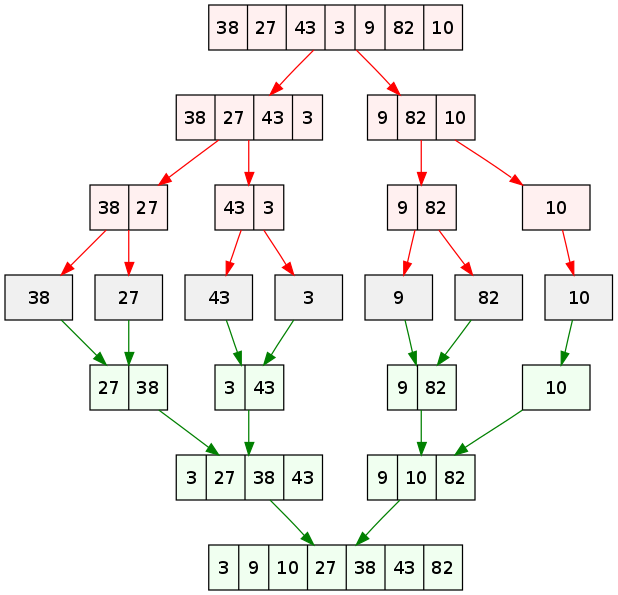
\includegraphics[width=0.7\textwidth]{mergesort.png}
        \caption{Fonte: \url{https://en.wikipedia.org/wiki/Merge_sort}}
    \end{figure}
    
\end{frame}

%%%%%%%%%%%%%%%%%%%%%%%%%%%%%%%%%%%%
\begin{frame}[fragile]{Merge Sort}

    \begin{minted}{c}
        void mergeSort(int vet[], int ini, int fim) {
            if (fim <= ini)
                return;
        
            int meio = (ini + fim)/2;
            mergeSort(vet, ini, meio);
            mergeSort(vet, meio+1, fim);
            intercala(vet, ini, meio, fim);            
        }
    \end{minted}

\end{frame}

%%%%%%%%%%%%%%%%%%%%%%%%%%%%%%%%%%%%
\begin{frame}[fragile]{Merge Sort}

    Com as funções anteriores podemos executar o exemplo:
    \vspace{-1em}
    \begin{minted}[fontsize=\scriptsize]{c}
        int main() {
            int vetor[10] = {14,7,8,34,56,4,0,9,-8,100};
            int i;

            printf("Vetor Antes: (%d", vetor[0]);
            for (i = 1; i < 10; i++)
                printf(", %d", vetor[i]);
            printf(")\n");

            mergeSort(vetor, 0, 9);

            printf("Vetor Depois: (%d", vetor[0]);
            for (i = 1; i < 10; i++)
                printf(", %d", vetor[i]);
            printf(")\n");

            return 0;
        }
    \end{minted}

\end{frame}

%%%%%%%%%%%%%%%%%%%%%%%%%%%%%%%%%%%%
%%%%%%%%%%%%%%%%%%%%%%%%%%%%%%%%%%%%
%%%%%%%%%%%%%%%%%%%%%%%%%%%%%%%%%%%%
%%%%%%%%%%%%%%%%%%%%%%%%%%%%%%%%%%%%
%%%%%%%%%%%%%%%%%%%%%%%%%%%%%%%%%%%%
%%%%%%%%%%%%%%%%%%%%%%%%%%%%%%%%%%%%
\section{Exercícios}

%%%%%%%%%%%%%%%%%%%%%%%%%%%%%%%%%%%%
\begin{frame}[fragile]{\exercicio}
    
    Altere os algoritmos vistos nesta aula para que estes ordenem um vetor de inteiros em ordem decrescente ao invés de ordem crescente.

\end{frame}

%%%%%%%%%%%%%%%%%%%%%%%%%%%%%%%%%%%%
\begin{frame}[fragile]{\exercicio}
    
    No algoritmo \cod{selectionSort}, o laço principal é executado de 0 até \cod{tam-2} e não \cod{tam-1}.
    Por quê?

\end{frame}

%%%%%%%%%%%%%%%%%%%%%%%%%%%%%%%%%%%%
%%%%%%%%%%%%%%%%%%%%%%%%%%%%%%%%%%%%
%%%%%%%%%%%%%%%%%%%%%%%%%%%%%%%%%%%%
%%%%%%%%%%%%%%%%%%%%%%%%%%%%%%%%%%%%
%%%%%%%%%%%%%%%%%%%%%%%%%%%%%%%%%%%%
%%%%%%%%%%%%%%%%%%%%%%%%%%%%%%%%%%%%
\section{Informações extras: outros algoritmos famosos de ordenação}

%%%%%%%%%%%%%%%%%%%%%%%%%%%%%%%%%%%%
%%%%%%%%%%%%%%%%%%%%%%%%%%%%%%%%%%%%
%%%%%%%%%%%%%%%%%%%%%%%%%%%%%%%%%%%%
\subsection{Insertion Sort}

%%%%%%%%%%%%%%%%%%%%%%%%%%%%%%%%%%%%
\begin{frame}[fragile]{Insertion Sort}

    \begin{itemize}
        \item Seja \cod{vet} um vetor contendo números inteiros, que devemos deixar ordenado.
        \item A ideia do algoritmo é a seguinte:
        \begin{itemize}
            \item A cada passo, uma porção de $0$ até $i-1$ do vetor já está ordenada.
            \item Devemos inserir o item da posição $i$ na posição correta para deixar o vetor ordenado até a posição $i$.
            \item No passo seguinte poderemos então consider que o vetor está ordenado até $i$.
        \end{itemize}
    \end{itemize}

\end{frame}

%%%%%%%%%%%%%%%%%%%%%%%%%%%%%%%%%%%%
\begin{frame}[fragile]{Insertion Sort}

    Exemplo: (5,3,2,1,90,6).

    O valor sublinhado representa onde está o índice $i$:\\
    $(5,{\color{blue}\underline{3}},2,1,90,6)$ : vetor ordenado de $0-0$.\\
    $(3,5,{\color{blue}\underline{2}},1,90,6)$ : vetor ordenado de $0-1$.\\
    $(2,3,5,{\color{blue}\underline{1}},90,6)$ : vetor ordenado de $0-2$.\\
    $(1,2,3,5,{\color{blue}\underline{90}},6)$ : vetor ordenado de $0-3$.\\
    $(1,2,3,5,90,{\color{blue}\underline{6}})$ : vetor ordenado de $0-4$.\\
    $(1,2,3,5,6,90)$ : vetor ordenado de $0-5$.

\end{frame}

%%%%%%%%%%%%%%%%%%%%%%%%%%%%%%%%%%%%
\begin{frame}[fragile]{Insertion Sort}

    \begin{itemize}
        \item Vamos supor que o vetor está ordenado de $0$ até $i-1$.
        \item Vamos inserir o elemento da posição $i$ no lugar correto.
    \end{itemize}

    \begin{minted}{c}
        j = i;
        while (j > 0) {
            /* trocar v[i] com elementos anteriores até achar sua posicao correta relativa a esses elementos */
            if (vet[j-1] > vet[j]) {
                troca(&vet[j], &vet[j-1]);
                j--;
            } else {
                break;
            }
        }
    \end{minted}

\end{frame}

%%%%%%%%%%%%%%%%%%%%%%%%%%%%%%%%%%%%
\begin{frame}[fragile]{Insertion Sort}

    Código completo:
    \vspace{-1em}
    \begin{minted}[fontsize=\scriptsize]{c}
        void insertionSort(int vet[], int tam) {
            int i, j;

            for (i = 1; i < tam; i++) {
                /* Colocar elemento v[i] na pos. correta */
                j = i;
                while (j > 0) {
                    /* trocar v[i] com elementos anteriores até achar sua posicao correta relativa a esses elementos */
                    if (vet[j-1] > vet[j]) {
                        troca(&vet[j], &vet[j-1]);
                        j--;
                    } else {
                        break;
                    }
                }
            }
        }
    \end{minted}

\end{frame}

%%%%%%%%%%%%%%%%%%%%%%%%%%%%%%%%%%%%
\begin{frame}[fragile]{Insertion Sort}

    \begin{itemize}
        \item Vamos apresentar uma forma alternativa de colocar \cod{v[i]} na posição correta.
        \item Vamos supor que o vetor está ordenado de $0$ até $i-1$.
        \item Vamos inserir o elemento da posição $i$ no lugar correto.
    \end{itemize}
    \vspace{-1em}
    \begin{minted}[fontsize=\scriptsize]{c}
        aux = vet[i];  /* precisamos inserir aux na posição correta */
        j = i - 1;     /* vamos analisar elementos das posições anteriores, a começar por i-1 */
        
        while (j >= 0 && vet[j] > aux) {
            /* enquanto vet[j] > aux, "empurra" vet[j] para a direita */
            vet[j+1] = vet[j];
            j--;
        }

        /* Nesse ponto, OU j = -1 OU vet[j] <= aux
           De qualquer forma, j+1 é a posição correta para vet[i] (aux) */
        vet[j+1] = aux;
    \end{minted} 

\end{frame}

%%%%%%%%%%%%%%%%%%%%%%%%%%%%%%%%%%%%
\begin{frame}[fragile]{Insertion Sort}

    Exemplo $(1, 3, 5, 10, 20, {\color{red}2^*}, 4)$ com $i=5$.

    $(1, 3, 5, 10, {\color{blue}\underline{20}}, 2, 4)$: \cod{aux} = 2; \cod{j} = 4; \\
    $(1, 3, 5, {\color{blue}\underline{10}}, 20, 20, 4)$: \cod{aux} = 2; \cod{j} = 3; \\
    $(1, 3, {\color{blue}\underline{5}}, 10, 10, 20, 4)$: \cod{aux} = 2; \cod{j} = 2; \\
    $(1, {\color{blue}\underline{3}}, 5, 5, 10, 20, 4)$: \cod{aux} = 2; \cod{j} = 1; \\
    $({\color{blue}\underline{1}}, 3, 3, 5, 10, 20, 4)$: \cod{aux} = 2; \cod{j} = 0; \\
    Aqui temos que \cod{vet[j] < aux}, logo, fazemos \cod{vet[j+1] = aux}\\
    $(1, 2, 3, 5, 10, 20, 4)$: \cod{aux} = 2; \cod{j} = 0; \\

\end{frame}

%%%%%%%%%%%%%%%%%%%%%%%%%%%%%%%%%%%%
\begin{frame}[fragile]{Insertion Sort}

    Código completo.
    \vspace{-1em}
    \begin{minted}[fontsize=\scriptsize]{c}
        void insertionSort(int vet[], int tam) {
            int i, j, aux;

            for (i = 1; i < tam; i++) {
                /* Assuma vetor ordenado de 0 até i-1 */
                aux = vet[i];
                j = i-1;

                while (j >= 0 && vet[j] > aux) {
                    /* Coloca elementos v[j] > v[i] para a direita */
                    vet[j+1] = vet[j];
                    j--;
                }

                vet[j+1] = aux; /* coloca v[i] na pos. correta */
            }
        }
    \end{minted}

\end{frame}

%%%%%%%%%%%%%%%%%%%%%%%%%%%%%%%%%%%%
%%%%%%%%%%%%%%%%%%%%%%%%%%%%%%%%%%%%
%%%%%%%%%%%%%%%%%%%%%%%%%%%%%%%%%%%%
\subsection{BubbleSort}

%%%%%%%%%%%%%%%%%%%%%%%%%%%%%%%%%%%%
\begin{frame}[fragile]{BubbleSort}
    
    \begin{itemize}
        \item Seja \cod{vet} um vetor contendo números inteiros.
        \item Devemos deixar \cod{vet} em ordem crescente.
        \item O algoritmo começa fazendo o seguinte:
        \begin{itemize}
            \item Compare \cod{vet[0]} com \cod{vet[1]} e troque-os se \cod{vet[0] > vet[1]}.
            \item Compare \cod{vet[1]} com \cod{vet[2]} e troque-os se \cod{vet[1] > vet[2]}.
            \item \ldots
            \item Compare \cod{vet[tam-2]} com \cod{vet[tam-1]} e troque-os se \cod{vet[tam-2] > vet[tam-1]}.
        \end{itemize}
        \item Após uma iteração repetindo estes passos o que podemos garantir?
        \begin{itemize}
            \item Que o maior elemento estará na posição correta!
        \end{itemize}
    \end{itemize}

\end{frame}

%%%%%%%%%%%%%%%%%%%%%%%%%%%%%%%%%%%%
\begin{frame}[fragile]{BubbleSort}

    \begin{itemize}
        \item Após uma iteração de trocas, o maior elemento estará na última posição.
        \item Após outra iteração de trocas, o segundo maior elemento estará na posição correta.
        \item E assim sucessivamente.
        \item Quantas iterações repetindo estas trocas precisamos para deixar o vetor ordenado?
    \end{itemize}

\end{frame}

%%%%%%%%%%%%%%%%%%%%%%%%%%%%%%%%%%%%
\begin{frame}[fragile]{BubbleSort}

    Exemplo: (5,3,2,1,90,6).

    Valores sublinhados estão sendo comparados:\\
    $({\color{red}\underline{5}},{\color{red}\underline{3}},2,1,90,6)$\\
    $(3,{\color{red}\underline{5}},{\color{red}\underline{2}},1,90,6)$\\
    $(3,2,{\color{red}\underline{5}},{\color{red}\underline{1}},90,6)$\\
    $(3,2,1,{\color{red}\underline{5}},{\color{red}\underline{90}},6)$\\
    $(3,2,1,5,{\color{red}\underline{90}},{\color{red}\underline{6}})$\\
    $(3,2,1,5,6,90)$
    
    \begin{itemize}
        \item Isto termina a primeira iteração de trocas.
        \item Temos que repetir todo o processo mais 4 vezes!
        \item Mas note que não precisamos mais avaliar a última posição.
    \end{itemize}

\end{frame}

%%%%%%%%%%%%%%%%%%%%%%%%%%%%%%%%%%%%
\begin{frame}[fragile]{BubbleSort}

    \begin{itemize}
        \item O código abaixo realiza as trocas de uma iteração.
        \item São comparados e trocados os elementos das posições: 0 e 1, 1 e 2, $\ldots$, $i-1$ e $i$.
        \item Assumimos que de $(i+1)$ até $(tam-1)$ o vetor já está com os maiores elementos ordenados.
     \end{itemize}

     \begin{minted}{c}
        for (j = 0; j < i; j++)
            if (vet[j] > vet[j+1])
                troca(&vet[j], &vet[j+1]);
    \end{minted}

\end{frame}

%%%%%%%%%%%%%%%%%%%%%%%%%%%%%%%%%%%%
\begin{frame}[fragile]{BubbleSort}

    \begin{minted}{c}
        void bubbleSort(int vet[], int tam) {
            int i, j, aux;

            for (i = tam-1; i > 0; i--) {
                for (j = 0; j < i; j++) /* Troca até pos. i */
                    if (vet[j] > vet[j+1])
                        troca(&vet[j], &vet[j+1]);
            }
        }
    \end{minted}

\end{frame}

%%%%%%%%%%%%%%%%%%%%%%%%%%%%%%%%%%%%
\begin{frame}[fragile]{BubbleSort}

    \begin{itemize}
        \item Note que as trocas na primeira iteração ocorrem até a última posição.
        \item Na segunda iteração ocorrem até a penúltima posição.
        \item E assim sucessivamente.
        \item Por quê?
    \end{itemize}

\end{frame}

%%%%%%%%%%%%%%%%%%%%%%%%%%%%%%%%%%%%%%%%%%%%%
%%%%%%%%%%%%%%%%%%%%%%%%%%%%%%%%%%%%%%%%%%%%%
%%%%%%%%%%%%%%%%%%%%%%%%%%%%%%%%%%%%%%%%%%%%%
%%%%%%%%%%%%%%%%%%%%%%%%%%%%%%%%%%%%%%%%%%%%%
%%%%%%%%%%%%%%%%%%%%%%%%%%%%%%%%%%%%%%%%%%%%%
%%%%%%%%%%%%%%%%%%%%%%%%%%%%%%%%%%%%%%%%%%%%%
\section{Informações extras: o problema da busca}

%%%%%%%%%%%%%%%%%%%%%%%%%%%%%%%%%%%%
\begin{frame}[fragile]{O problema da busca}

    \begin{block}{}
        Temos uma coleção de elementos, onde cada elemento possui um identificador/chave único, e recebemos uma chave para busca.
        Devemos encontrar o elemento da coleção que possui a mesma chave ou identificar que não existe nenhum elemento com a chave dada.
    \end{block}

    Nos nossos exemplos usaremos um vetor de inteiros como a coleção.

    O valor da chave será o próprio valor de cada número.

    Apesar de usarmos inteiros, os algoritmos servem para buscar elementos em qualquer coleção de elementos que possuam chaves que possam ser comparadas, como registros com algum campo de identificação único (RA, ou RG, ou CPF, etc.).

\end{frame}

%%%%%%%%%%%%%%%%%%%%%%%%%%%%%%%%%%%%
\begin{frame}[fragile]{O Problema da busca}

    \begin{itemize}
        \item O problema da busca é um dos mais básicos em computação e também possui diversas aplicações.
        \begin{itemize}
            \item Suponha que temos um cadastro com registros de motoristas.
            \item Um vetor de registros é usado para armazenar as informações dos motoristas. Podemos usar como chave o número da carteira de motorista, ou o RG, ou o CPF.
        \end{itemize}
        \item Veremos algoritmos simples para realizar a busca assumindo que dados estão em um vetor.
        \item Em disciplinas mais avançadas são estudados outros algoritmos e estruturas (que não um vetor) para armazenar e buscar elementos.
    \end{itemize}

\end{frame}

%%%%%%%%%%%%%%%%%%%%%%%%%%%%%%%%%%%%%%%%%%%%%
\begin{frame}[fragile]{O Problema da busca}

    \begin{itemize}
        \item Nos nossos exemplos vamos criar a função\\
        \cod{int busca(int vet[], int tam, int chave)}\\
        que recebe um vetor com um determinado tamanho, e uma chave para busca.
        \item A função deve retornar o índice do vetor que contém a chave ou -1 caso a chave não esteja no vetor.
    \end{itemize}

\end{frame}

%%%%%%%%%%%%%%%%%%%%%%%%%%%%%%%%%%%%%%%%%%%%%
\begin{frame}[fragile]{O Problema da busca}

    \begin{center}
        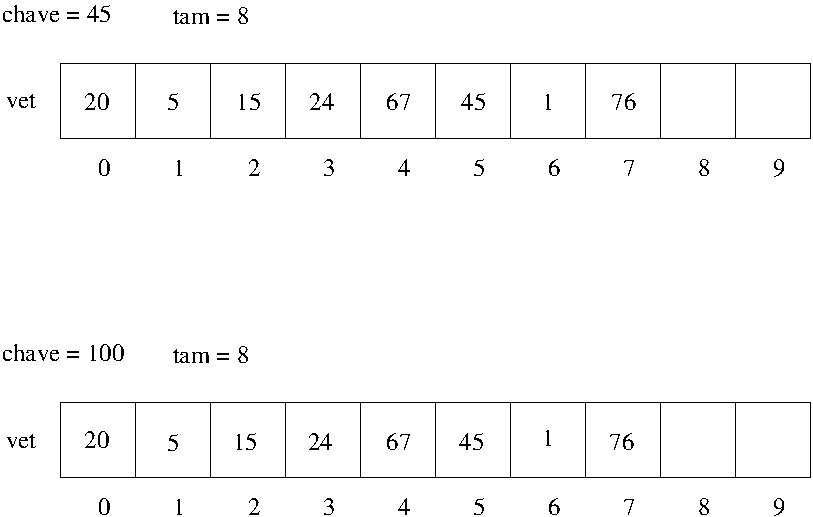
\includegraphics[scale=0.5]{busca}
    \end{center}

    No exemplo mais acima, a função deve retornar 5, enquanto no exemplo mais abaixo a função deve retornar -1.

\end{frame}

%%%%%%%%%%%%%%%%%%%%%%%%%%%%%%%%%%%%
%%%%%%%%%%%%%%%%%%%%%%%%%%%%%%%%%%%%
%%%%%%%%%%%%%%%%%%%%%%%%%%%%%%%%%%%%
\subsection{Busca sequencial}

%%%%%%%%%%%%%%%%%%%%%%%%%%%%%%%%%%%%
\begin{frame}[fragile]{Busca sequencial}

    \begin{itemize}
        \item A busca sequencial é o algoritmo mais simples de busca:
        \begin{itemize}
            \item Percorra todo o vetor comparando a chave com o valor de cada posição.
            \item Se for igual para alguma posição, então devolva esta posição.
            \item Se o vetor todo foi percorrido então devolva -1.
        \end{itemize}
    \end{itemize}

\end{frame}

%%%%%%%%%%%%%%%%%%%%%%%%%%%%%%%%%%%%
\begin{frame}[fragile]{Busca sequencial}

    \begin{minted}{c}
        int buscaSequencial(int vet[], int tam, int chave) {
            int i;
            for (i = 0; i < tam; i++) {
                if (vet[i] == chave)
                    return i;
            }
            return -1;
        }
    \end{minted}

\end{frame}

%%%%%%%%%%%%%%%%%%%%%%%%%%%%%%%%%%%%
\begin{frame}[fragile]{Busca sequencial}

    \vspace{-1em}
    \begin{minted}[fontsize=\footnotesize]{c}
        #include <stdio.h>
        int buscaSequencial(int vet[], int tam, int chave);
        int main() {
            int pos, vet[] = {20, 5, 15, 24, 67, 45, 1, 76};
            
            pos = buscaSequencial(vet, 8, 45);
            if (pos != -1)
                printf("A posicao da chave 45 no vetor é: %d\n", pos);
            else
                printf("A chave 45 não está no vetor!\n");

            pos = buscaSequencial(vet, 8, 100);
            if (pos != -1)
                printf("A posicao da chave 100 no vetor é: %d\n", pos);
            else
                printf("A chave 100 não está no vetor!\n");

            return 0;
        }
    \end{minted} 

\end{frame}

%%%%%%%%%%%%%%%%%%%%%%%%%%%%%%%%%%%%
%%%%%%%%%%%%%%%%%%%%%%%%%%%%%%%%%%%%
%%%%%%%%%%%%%%%%%%%%%%%%%%%%%%%%%%%%
\subsection{Busca binária}

%%%%%%%%%%%%%%%%%%%%%%%%%%%%%%%%%%%%
\begin{frame}[fragile]{Busca binária}

    \begin{itemize}
        \item A busca binária é um algoritmo um pouco mais sofisticado.
        \item É mais eficiente (tempo), mas requer que o vetor esteja ordenado pelos valores da chave de busca.
        \item A ideia do algoritmo é a seguinte (assuma que o vetor está ordenado):
        \begin{itemize}
            \item Verifique se a chave de busca é igual ao valor da posição do meio do vetor.
            \item Caso seja igual, devolva esta posição.
            \item Caso o valor desta posição seja maior, então repita o processo mas considere que o vetor tem metade do tamanho, indo até a posição anterior a do meio.
            \item Caso o valor desta posição seja menor, então repita o processo mas considere que o vetor tem metade do tamanho e inicia na posição seguinte a do meio.
        \end{itemize}
    \end{itemize}

\end{frame}

%%%%%%%%%%%%%%%%%%%%%%%%%%%%%%%%%%%%
\begin{frame}[fragile]{Busca binária}

    Pseudocódigo:
    \begin{minted}{bash}
        /* vetor começa em ini e termina em fim */
        ini = 0
        fim = tam-1

        Repita enquanto tamanho do vetor considerado for >= 1:
            meio = (ini + fim)/2
            Se vet[meio] == chave Então
                devolva meio
            Se vet[meio] > chave Então
                fim = meio - 1
            Se vet[meio] < chave Então
                ini = meio + 1
    \end{minted}

\end{frame}

%%%%%%%%%%%%%%%%%%%%%%%%%%%%%%%%%%%%%%%%%%%%%
\begin{frame}[fragile]{Busca binária}

    \begin{center}
        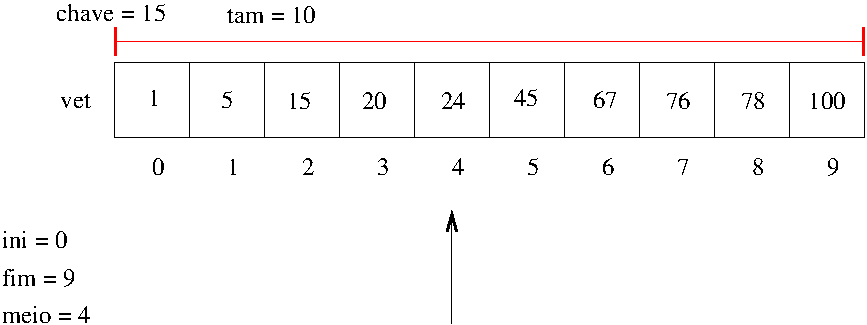
\includegraphics[scale=0.7]{buscaBin}
    \end{center}

    Como o valor da posição do meio é maior que a chave, atualizamos \cod{fim} do vetor considerado.

\end{frame}

%%%%%%%%%%%%%%%%%%%%%%%%%%%%%%%%%%%%%%%%%%%%%
\begin{frame}[fragile]{Busca binária}

    \begin{center}
        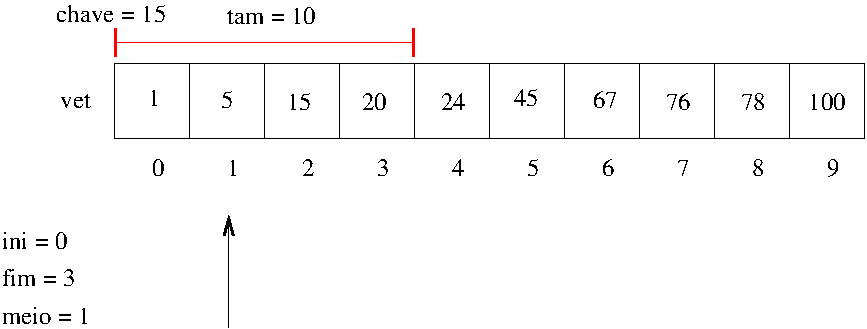
\includegraphics[scale=0.7]{buscaBin2}
    \end{center}

    Como o valor da posição do meio é menor que a chave, atualizamos \cod{ini} do vetor considerado.

\end{frame}

%%%%%%%%%%%%%%%%%%%%%%%%%%%%%%%%%%%%%%%%%%%%%
\begin{frame}[fragile]{Busca binária}

    \begin{center}
        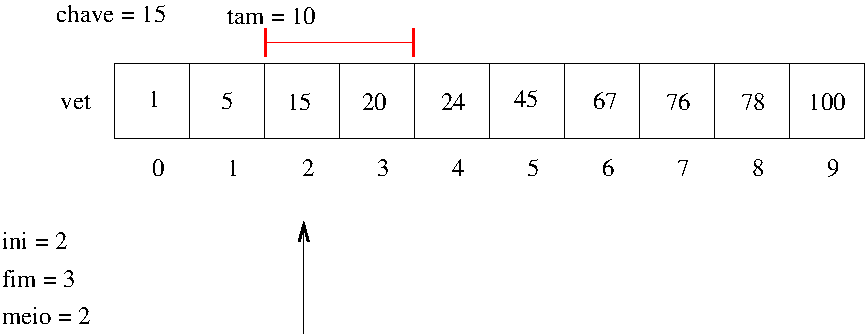
\includegraphics[scale=0.7]{buscaBin3}
    \end{center}

    Finalmente encontramos a chave e podemos devolver sua posição 2.

\end{frame}

%%%%%%%%%%%%%%%%%%%%%%%%%%%%%%%%%%%%
\begin{frame}[fragile]{Busca binária}

    Código completo:
    \vspace{-1em}
    \begin{minted}{c}
        int buscaBinaria(int vet[], int tam, int chave) {
            int ini = 0, fim = tam-1, meio;

            while (ini <= fim) { /* enquanto o vetor tiver pelo menos 1 elemento */
                meio = (ini+fim)/2;
                if (vet[meio] == chave)
                    return meio;
                else if (vet[meio] > chave)
                    fim = meio - 1;
                else
                    ini = meio + 1;
            }
            return -1;
        }
    \end{minted}

\end{frame}

%%%%%%%%%%%%%%%%%%%%%%%%%%%%%%%%%%%%
\begin{frame}[fragile]{Busca binária}

    Exemplo de uso:
    \vspace{-1em}
    \begin{minted}[fontsize=\scriptsize]{c}
        int main() {
            int vet[] = {20, 5, 15, 24, 67, 45, 1, 76, 78, 100};
            int pos, i;

            /* antes de usar a busca devemos ordenar o vetor */
            selectionSort(vet, 10);
            printf("Vetor Ordenado: (%d", vet[0]);
            for (i = 1; i < 10; i++)
                printf(", %d", vet[i]);
            printf(")\n");

            pos = buscaBinaria(vet, 10, 15);
            if (pos != -1)
                printf("A posicao da chave 15 no vetor é: %d\n", pos);
            else
                printf("A chave 15 não está no vetor!\n");

            return 0;
        }
    \end{minted} 

\end{frame}

%%%%%%%%%%%%%%%%%%%%%%%%%%%%%%%%%%%%
\begin{frame}[fragile]{Exercício}

    Refaça as funções de busca sequencial e busca binária assumindo que o vetor possui chaves que podem aparecer repetidas.
    
    Neste caso, você deve retornar em um outro vetor todas as posições onde a chave foi encontrada.

    Protótipo: \cod{int busca(int vet[], int tam, int chave, int *posicoes)}

    Você deve devolver em \cod{posicoes[]} as posições de \cod{vet} que possuem a \cod{chave}, e o retorno da função é o número de ocorrências da chave.

    \textbf{OBS:} O vetor \cod{posições} deve ser alocado dentro da função busca e ter espaço suficiente para guardar todas as possíveis ocorrências.

\end{frame}

%%%%%%%%%%%%%%%%%%%%%%%%%%%%%%%%%%%%
%%%%%%%%%%%%%%%%%%%%%%%%%%%%%%%%%%%%
%%%%%%%%%%%%%%%%%%%%%%%%%%%%%%%%%%%%
%%%%%%%%%%%%%%%%%%%%%%%%%%%%%%%%%%%%
%%%%%%%%%%%%%%%%%%%%%%%%%%%%%%%%%%%%
%%%%%%%%%%%%%%%%%%%%%%%%%%%%%%%%%%%%
\section{Informações extras: questões sobre eficiência}

%%%%%%%%%%%%%%%%%%%%%%%%%%%%%%%%%%%%
\begin{frame}[fragile]{Eficiência dos algoritmos}

    \begin{block}{}
        Podemos medir a eficiência de qualquer algoritmo analisando a quantidade de recursos (tempo, memória, banda de rede, etc.) que o algoritmo usa para resolver o problema para o qual foi proposto.
    \end{block}

    A forma mais simples é medir a eficiência em relação ao tempo.
    
    Para isso, analisamos quantas instruções um algoritmo usa para resolver o problema.

    Podemos fazer uma análise simplificada dos algoritmos de busca analisando a quantidade de vezes que os algoritmos {\bf acessam} uma posição do vetor.

\end{frame}

%%%%%%%%%%%%%%%%%%%%%%%%%%%%%%%%%%%%
\begin{frame}[fragile]{Eficiência dos algoritmos}

    No caso da busca sequencial existem três possibilidades:

    \begin{itemize}
        \item Na melhor das hipóteses a chave de busca estará na posição 0. Portanto teremos um único acesso em \cod{vet[0]}.
        \item Na pior das hipóteses, a chave é o último elemento ou não pertence ao vetor, e portanto acessaremos todas as \cod{tam} posições do vetor.
        \item É possível mostrar que se uma chave qualquer pode ser requisitada com a mesma probabilidade, então o número de acessos será \cod{(tam+1)/2} em média.
    \end{itemize}

\end{frame}

%%%%%%%%%%%%%%%%%%%%%%%%%%%%%%%%%%%%
\begin{frame}[fragile]{Eficiência dos algoritmos}

    No caso da busca binária temos também três possibilidades:

    \begin{itemize}
        \item Na melhor das hipóteses a chave de busca estará na posição do meio. Portanto teremos um único acesso.
        \item Na pior das hipóteses, teremos $(\log_2 \mbox{\cod{tam}})$ acessos.
        \begin{itemize}
            \item Para ver isso note que a cada verificação de uma posição do vetor, o tamanho do vetor considerado é dividido pela metade.
            No pior caso repetimos a busca até o vetor considerado ter tamanho 1. 
            Se você pensar um pouco, o número de acessos $x$ pode ser encontrado resolvendo-se a equação: $\frac{\mbox{\cod{tam}}}{2^x} = 1$, cuja solução é $x = (\log_2 \mbox{\cod{tam}})$.
        \end{itemize}
        \item É possível mostrar que se uma chave qualquer pode ser requisitada com a mesma probabilidade, então o número de acessos será $(\log_2 \mbox{\cod{tam}}) -1$ em média.
    \end{itemize}

\end{frame}

%%%%%%%%%%%%%%%%%%%%%%%%%%%%%%%%%%%%
\begin{frame}[fragile]{Eficiência dos algoritmos}

    Para se ter uma ideia da diferença de eficiência dos dois algoritmos, considere que temos um cadastro com $10^6$ (um milhão) de itens.

    \begin{itemize}
        \item Com a busca sequencial, a procura de um item qualquer gastará na média $(10^6 + 1)/2 \approx 500000$ acessos.
        \item Com a busca binária teremos $(\log_2 10^6) -1 \approx 20$ acessos.
    \end{itemize}

\end{frame}

%%%%%%%%%%%%%%%%%%%%%%%%%%%%%%%%%%%%
\begin{frame}[fragile]{Eficiência dos algoritmos}

    Mas uma ressalva deve ser feita: para utilizar a busca binária, o vetor precisa estar ordenado!

    \begin{itemize}
        \item Se você tiver um cadastro onde vários itens são removidos e inseridos com frequência, e a busca deve ser feita intercalada com estas operações, então a busca binária pode não ser a melhor opção, já que você precisará ficar mantendo o vetor ordenado.
        \item Caso o número de buscas feitas seja muito maior, quando comparado com outras operações, então a busca binária é uma boa opção. 
    \end{itemize}

\end{frame}

\end{document}
